\chapter{Testing and Evaluation}

To properly evaluate the system, multiple testing procedures were implemented.
These started with first testing the accuarcy of individual components on the \gls{pcb}, and then testing the probes ability to measure salinity, through voltage measurements relating to conductivity.
Additionally, tests were done on the \gls{ml} model programmed to map the salinity.

A summary of the tests and their outcomes can be seen in Table~\ref{table:test_summary}. %TODO


\section{Component and Equipment Testing}
Before the probe could be used to measure salinity, the accuarcy of its components needed to be tested.
These procedures were completed before the probe was encased in resin, as access to the circuitry was required.

\subsection{Resistor Testing}
For accurate electrode resistance to be measured, the the $R1$ parallel resistor combinations would need to be measured.
As shown in Section~\ref{sec:circuit_design}, by calculation, the $R1$ resistors should have equivalent resistances of $100\Omega$, $1K\Omega$ and $10K\Omega$, with an uncertainty of $\pm0.33\%$.
These were measured using the $Keysight Technologies U3401A$ multimeter, which had a resistance accuracy of $0.1\%$.
This multimeter would be used for all subsequent \gls{dc} voltage measurements, and has a voltage accuracy of $0.02\%$.
The multimeter probes had a resistance of $0.154\Omega$ which was accounted for.
The $R1$ resistors were measured and are shown in Table~\ref{table:resistance_test}.


\begingroup
    \renewcommand{\arraystretch}{1.8} % increase row height (adjust factor as needed)
    \begin{table}[h!]
        \centering
            \begin{tabular}{|>{\centering\arraybackslash}p{5cm}|
                >{\centering\arraybackslash}m{5cm}|}
            \hline
            Theoretical R ($\Omega$) & Meausured R ($\Omega$) \\ \hline
            $99.67-100.33$ & $99.888$ \\ \hline
            $996.7-1003.3$ & $1000.146$ \\ \hline
            $9967-10033$ & $10005.746$ \\ \hline
            \end{tabular}
        \caption{Table of $R_1$ resistor measurements}
        \label{table:resistance_test}
    \end{table}
\endgroup

The calibration resistor with an expected resistance of $5\Omega\pm0.25\%$ was measured to have a resistance of $5.142\Omega$.
Taking into account the probe resistance, the calibration resistor had a resistance of $4.988\Omega$.

\subsection{DAC and ADC Accuracy}
Both the accuracy of the \gls{dac} and \gls{adc} needed to be measured as these were used for the output and measurement, respectively.

The first test was done by programming the \gls{dac} to output from its minimum to maximum value.
This would allow for the evaluation of the \gls{dac}s output offset and gain to be measured.
The \gls{adc}s were also used to measure the output of the \gls{dac}, and these measurements were compared relative to the voltage measured by the multimeter.
Figure~\ref{fig:dac_test} shows the relationship between the voltage inputted to the \gls{dac}, and its output voltage, with the output measured on the multimeter.
Note that the reference voltage of the \gls{dac} was measured to be $5.001V$.

\begin{figure}[H]\label{fig:dac_test}
    \centering
    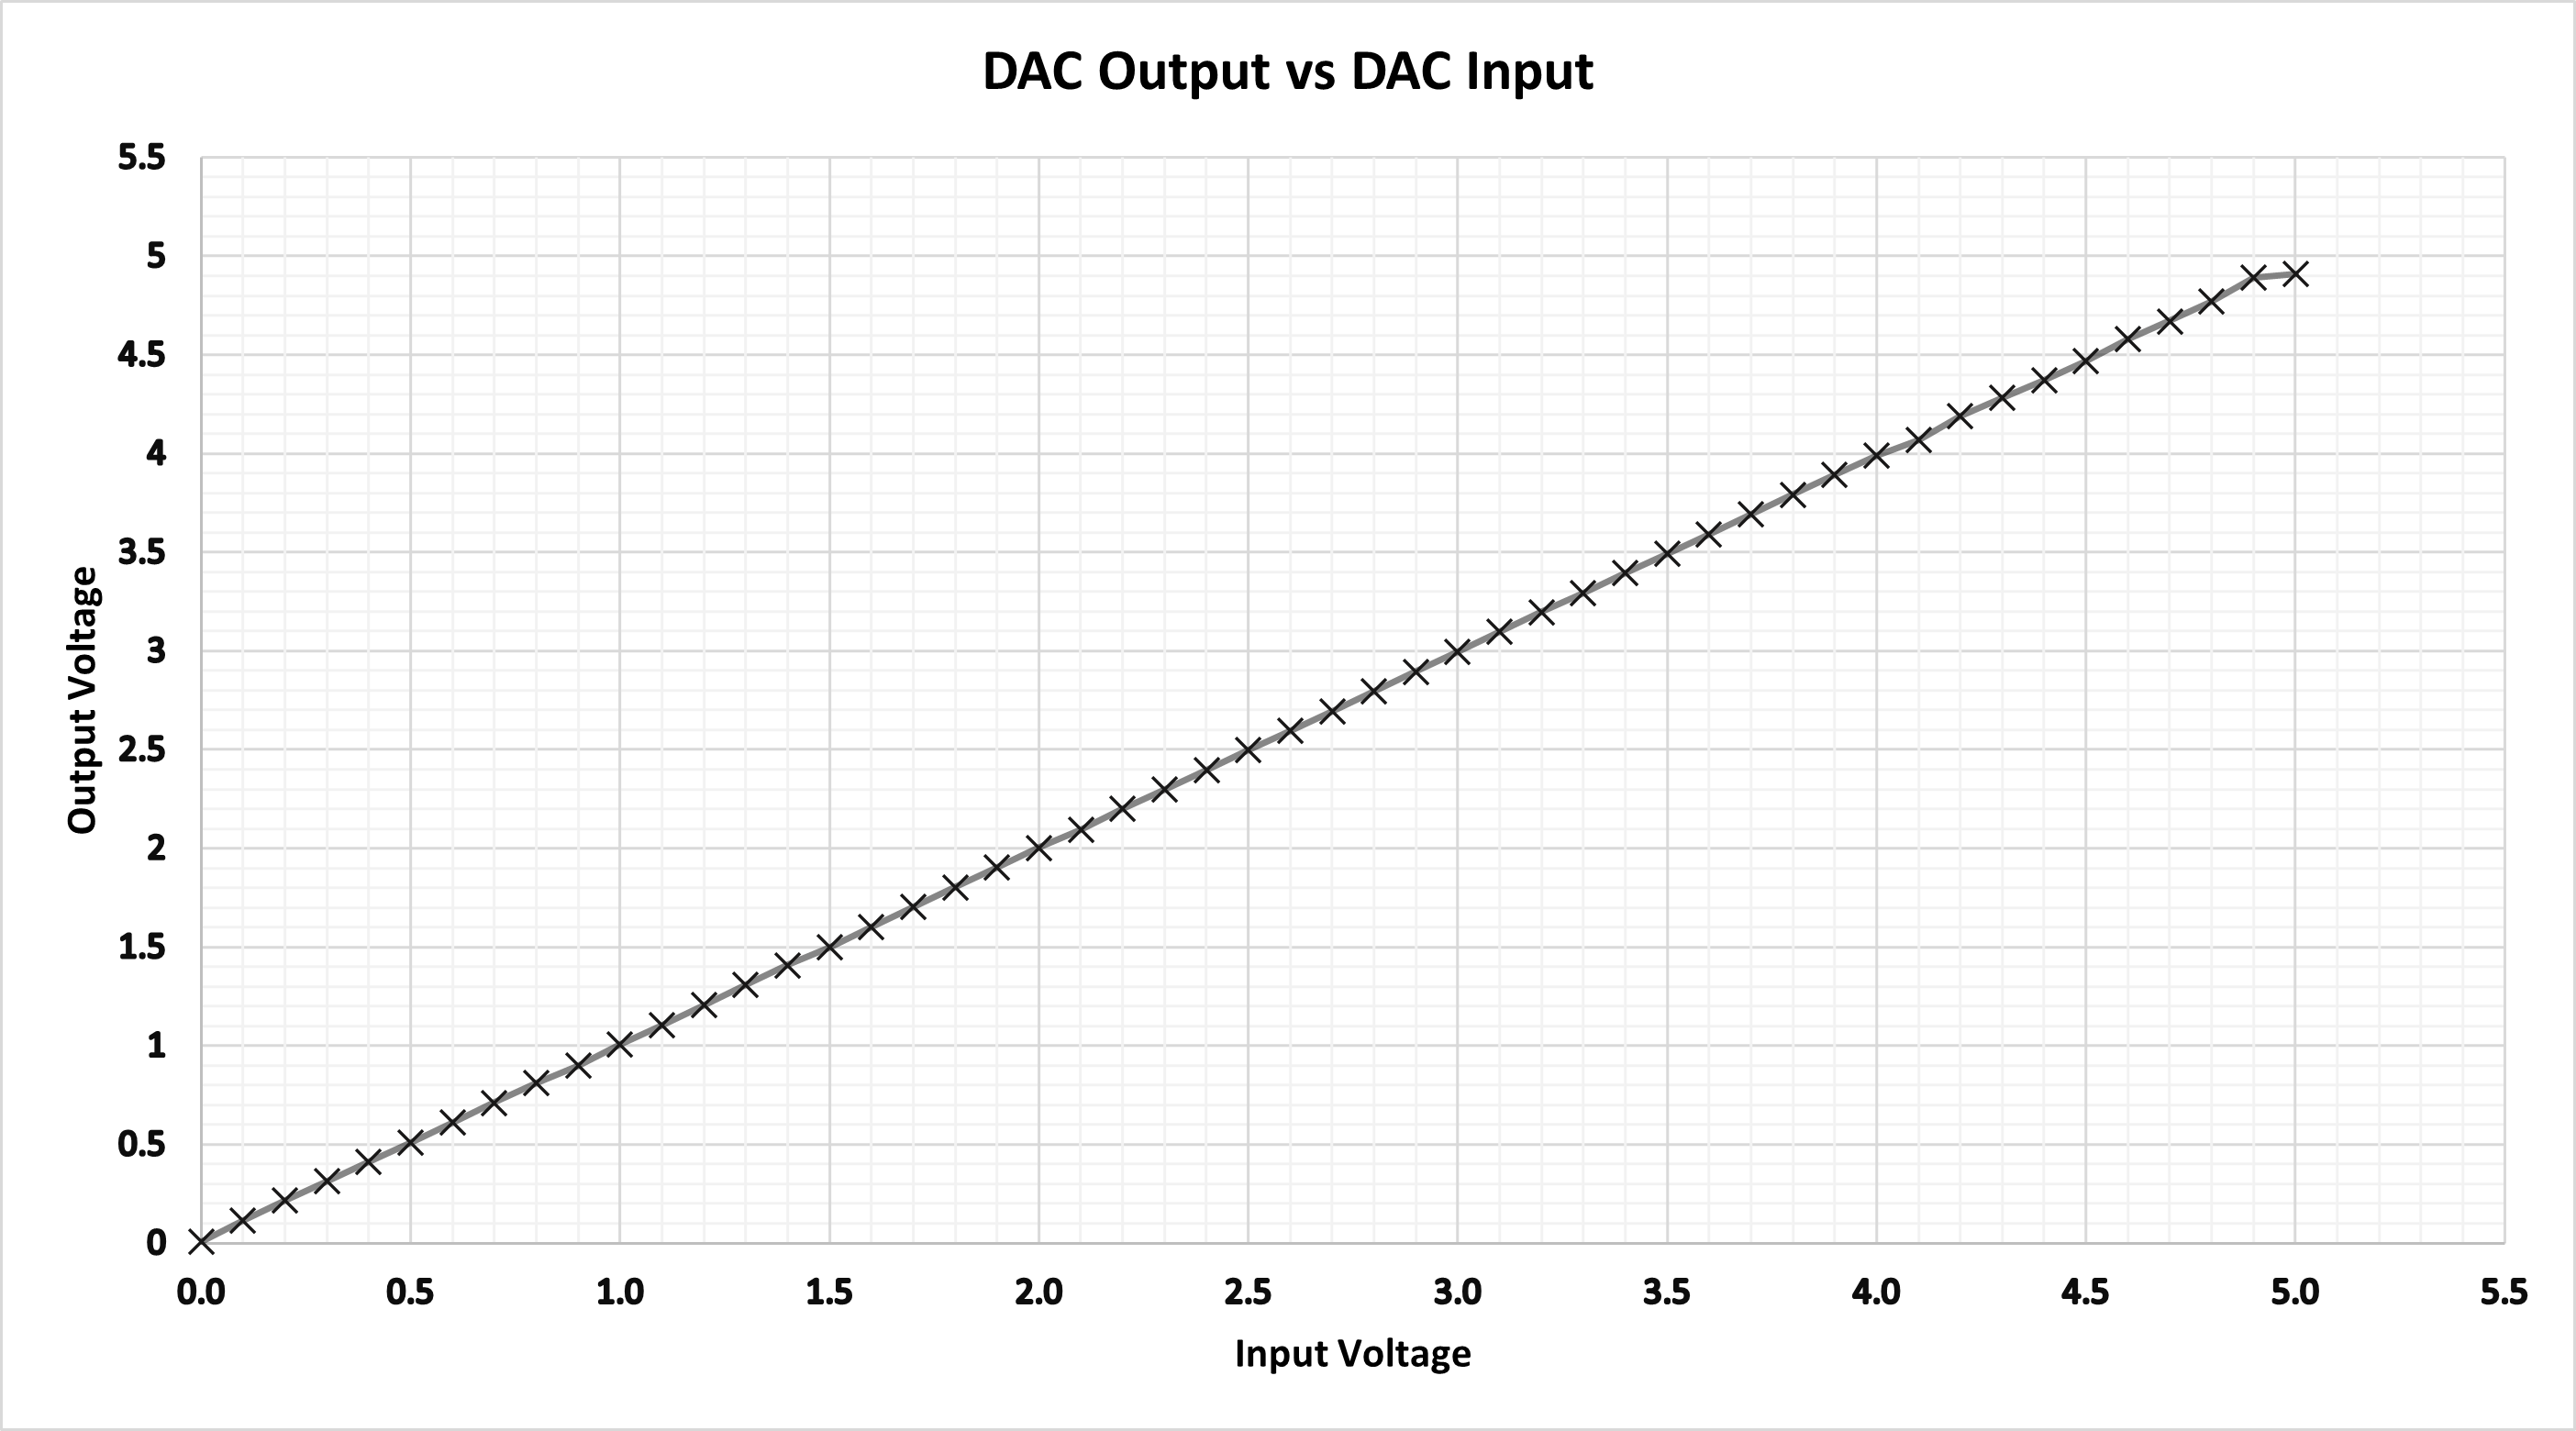
\includegraphics[width=0.7\textwidth]{figures/dac_test.png}
    \caption{DAC Output Voltage vs Input Voltage}
    \label{fig:dac_test}
\end{figure}

Based on the measurements made by the multimeter, the \gls{dac} had a output range of $0.0098V - 4.91V$, an offset of $0.0098V$ and gain of $0.98688$.

The accuracy of the \gls{adc} was then tested by comparing the \gls{dac} output measured by the \gls{adc} and multimeter.
Note, this \gls{adc} measurement was taken after the unity gain buffer op-amp.
For this test, the \gls{adc} took 5 measurements at each voltage step, which were taken at $1\mu{s}$ interval. 
These 5 values were averaged to give the voltage at that step.
The results of this test can be seen in Figure~\ref{fig:adc_test}.

\begin{figure}[H]\label{fig:adc_test}
    \centering
    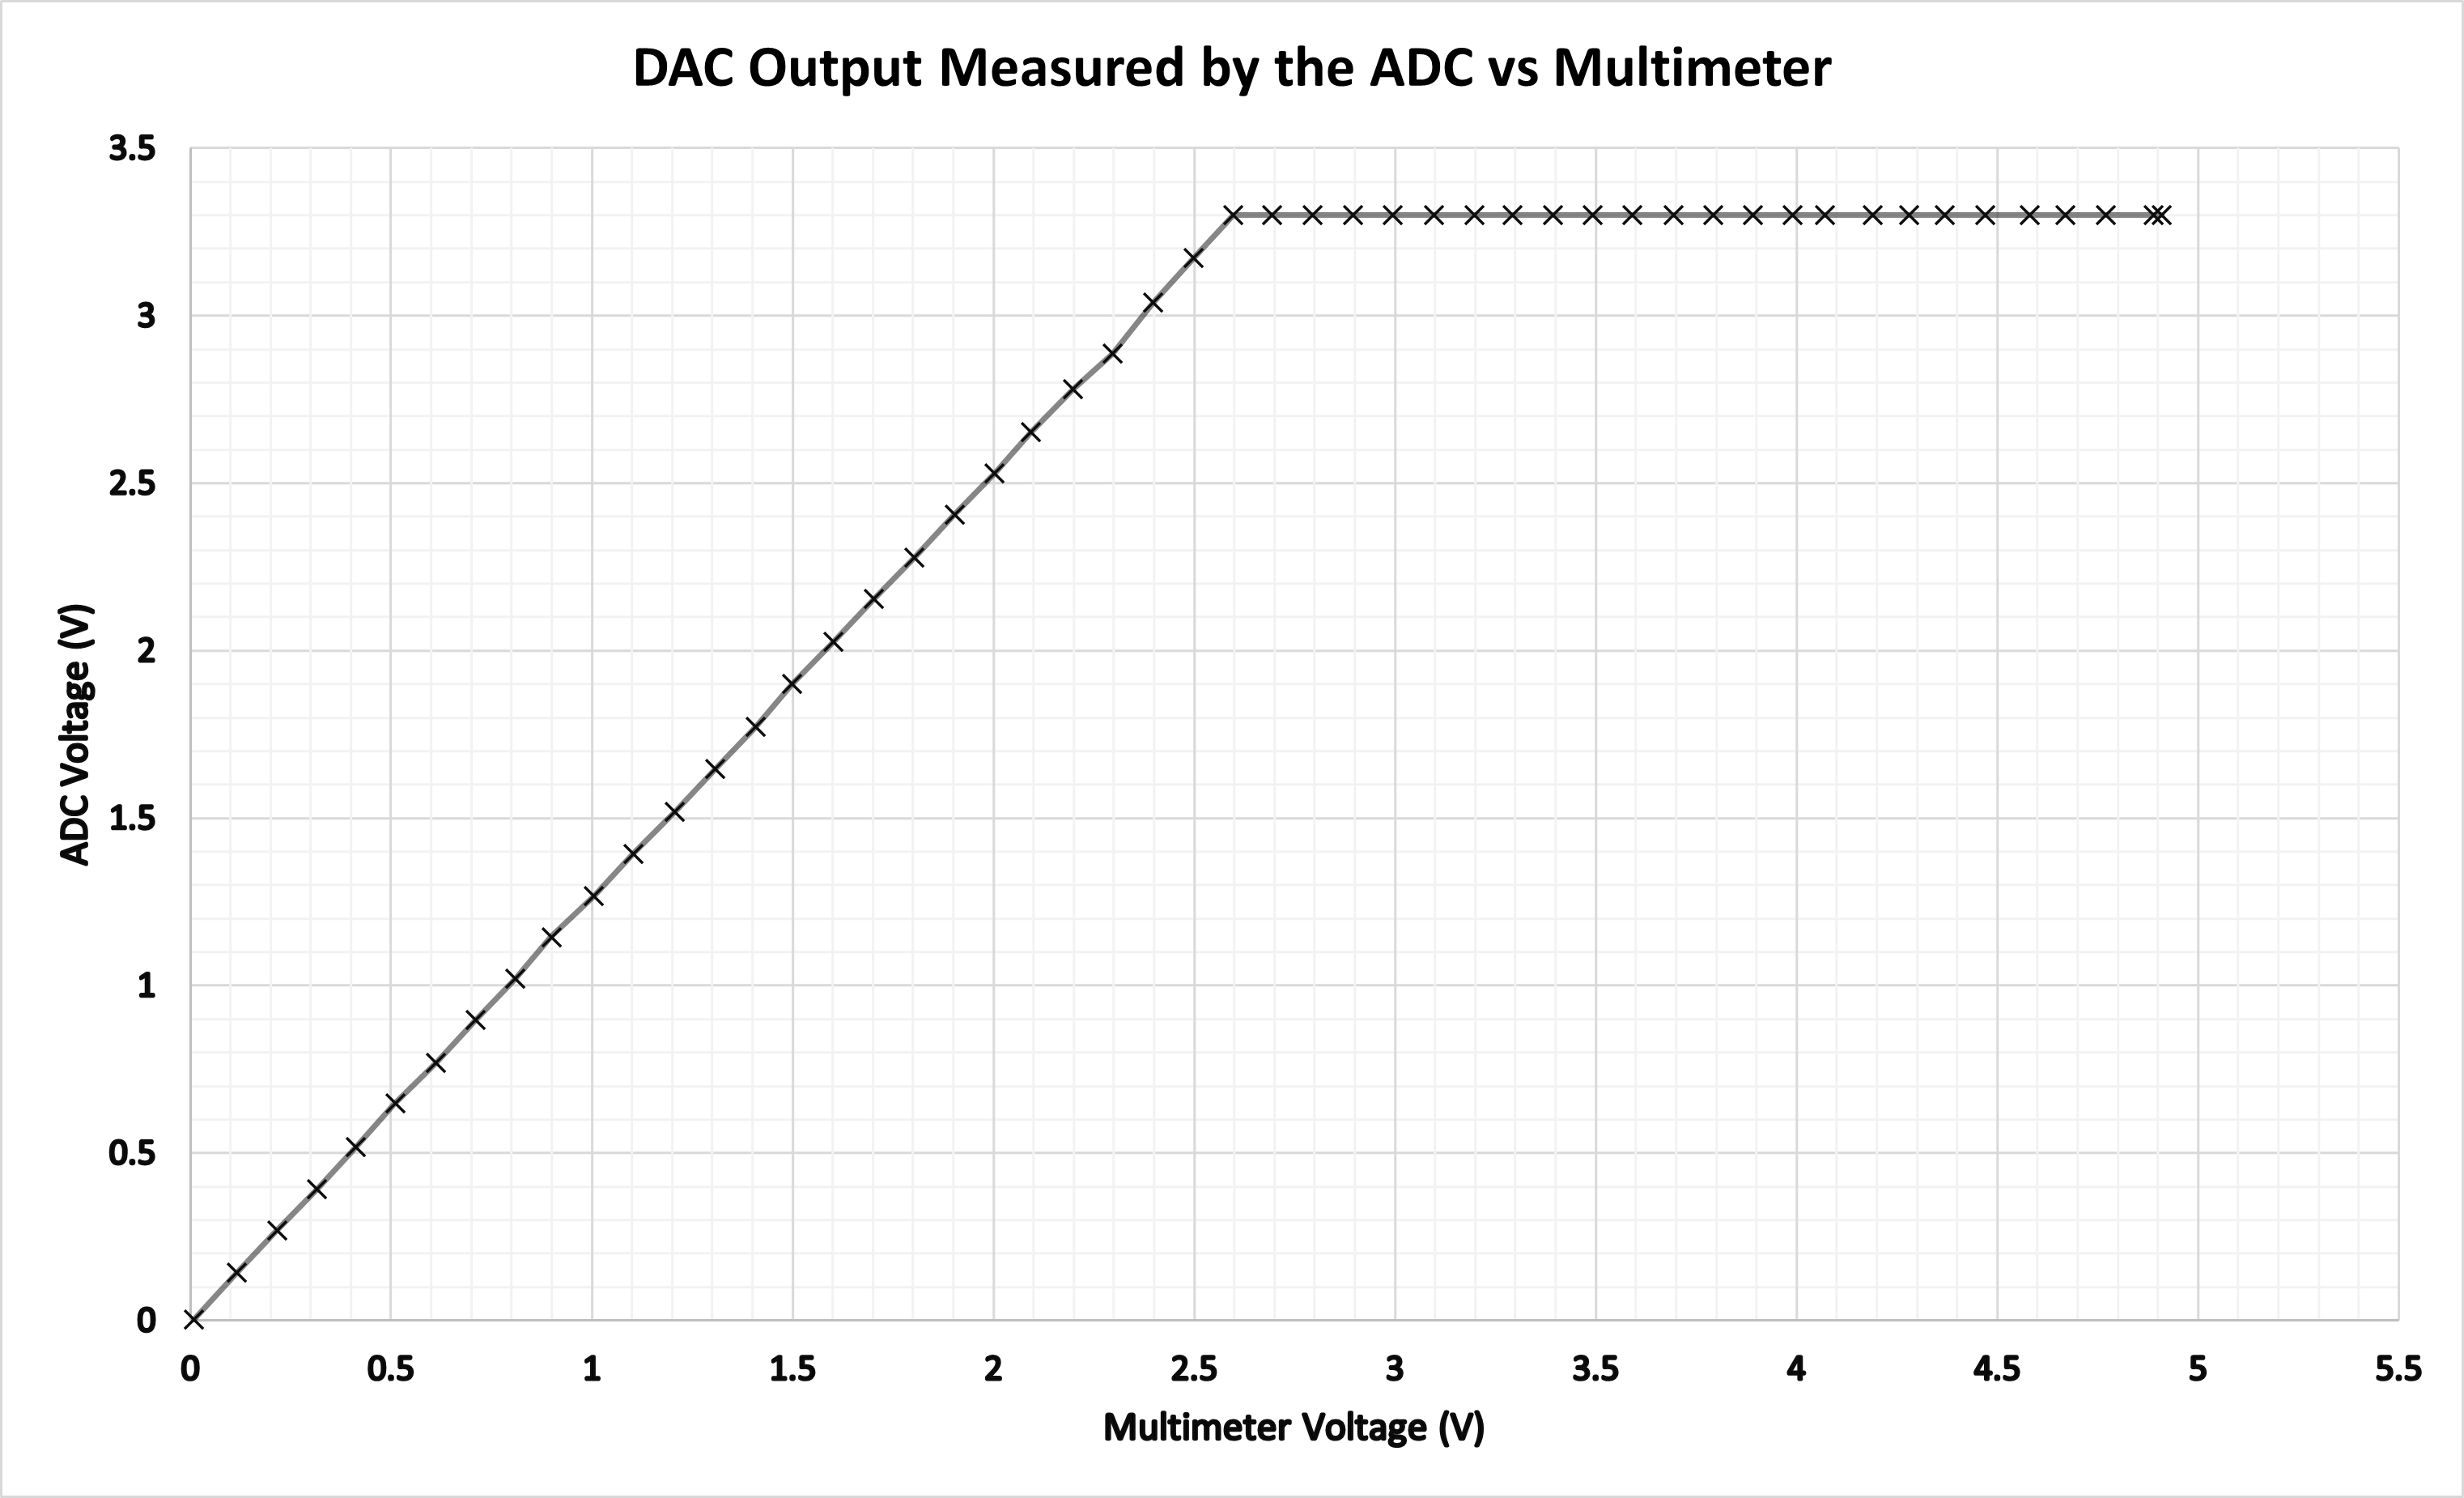
\includegraphics[width=0.7\textwidth]{figures/adc_test.png}
    \caption{DAC Output Measured by the ADC vs Multimeter}
    \label{fig:adc_test}
\end{figure}

Once the voltage measured by the \gls{adc} reaches $3.3V$ the \gls{adc} saturates as its reference voltage is $3.3V$.
The gain of the \gls{adc} was calculated to be 1.28072 compared to the mulimeter.

\subsection{Accuracy of Resistance Measuring Circuitry}\label{sec:resistor_measuring_test}
In order to evaluate the resistance circuit's ability to accurately measure resistance, resistors were attached to the electrode's solder pads.
This resistor acted as the $R2$ resistor and its value was calculated using Equation~\ref{eqn:resistance_divider}.
The resistance was calculated using the voltage sweep and single voltage functions mentioned in Section~\ref{sec:uc_program} with some slight adjustments for calculating resistance only.
These values were then compared to a multimeter measurement of the resistors, and the probe resistance taken into account.
Resistances were measured at $0\Omega$, or a short circuit, and then $10-82\Omega$ using resistors from the E12-Series, with an accuracy of $\pm5\%$
The $100\Omega$ $R1$ resistor was used.
The outcome of this test can be seen in Table~\ref{table:resistance_measurement_test}.

\begingroup
    \renewcommand{\arraystretch}{1.8} % increase row height (adjust factor as needed)
    \begin{table}[h!]
        \centering
            \begin{tabular}{|>{\centering\arraybackslash}p{4cm}|
                >{\centering\arraybackslash}m{5cm}|
                >{\centering\arraybackslash}m{6cm}|}
            \hline
                \textbf{Multimeter Resistance $\Omega$} & \textbf{Measured R $\Omega$} & \textbf{Acceptable Range $\Omega$} \\ \hline
                0 & 0 & 0-0 \\ \hline
                9.848 & 9.99578925 & 9.5-10.5 \\ \hline
                11.972 & 12.0007881 & 11.4-12.6 \\ \hline
                15.124 & 15.0062442 & 14.25-15.75 \\ \hline
                18.872 & 18.1212224 & 17.1-18.9 \\ \hline
                22.004 & 22.0162646 & 20.9-23.1 \\ \hline
                27.101 & 26.9989572 & 25.65-28.35 \\ \hline
                33.012 & 33.0181212 & 31.35-34.65 \\ \hline
                39.201 & 39.0305398 & 37.05-40.95 \\ \hline
                47.100 & 47.0431559 & 44.65-49.35 \\ \hline
                56.023 & 56.0306769 & 53.2-58.8 \\ \hline
                68.014 & 68.0599057 & 64.6-71.4 \\ \hline
                79.785 & 78.208607 & 77.9-86.1 \\ \hline
            \end{tabular}
        \caption{Table for Resistor Measurement Test}
        \textit{Note 1: For this test an input of 2V was used} \\
        \textit{Note 2: Accepectable range indicates resistance values due to $\pm5\%$ accuarcy}
        \label{table:resistance_measurement_test}
    \end{table}
\endgroup

The voltage sweep test, from 0-2V, achieved a similar measuring accuracy as seen in Figure~\ref{fig:resistance_measurement_test}
\begin{figure}[H]\label{fig:resistance_measurement_test}
    \centering
    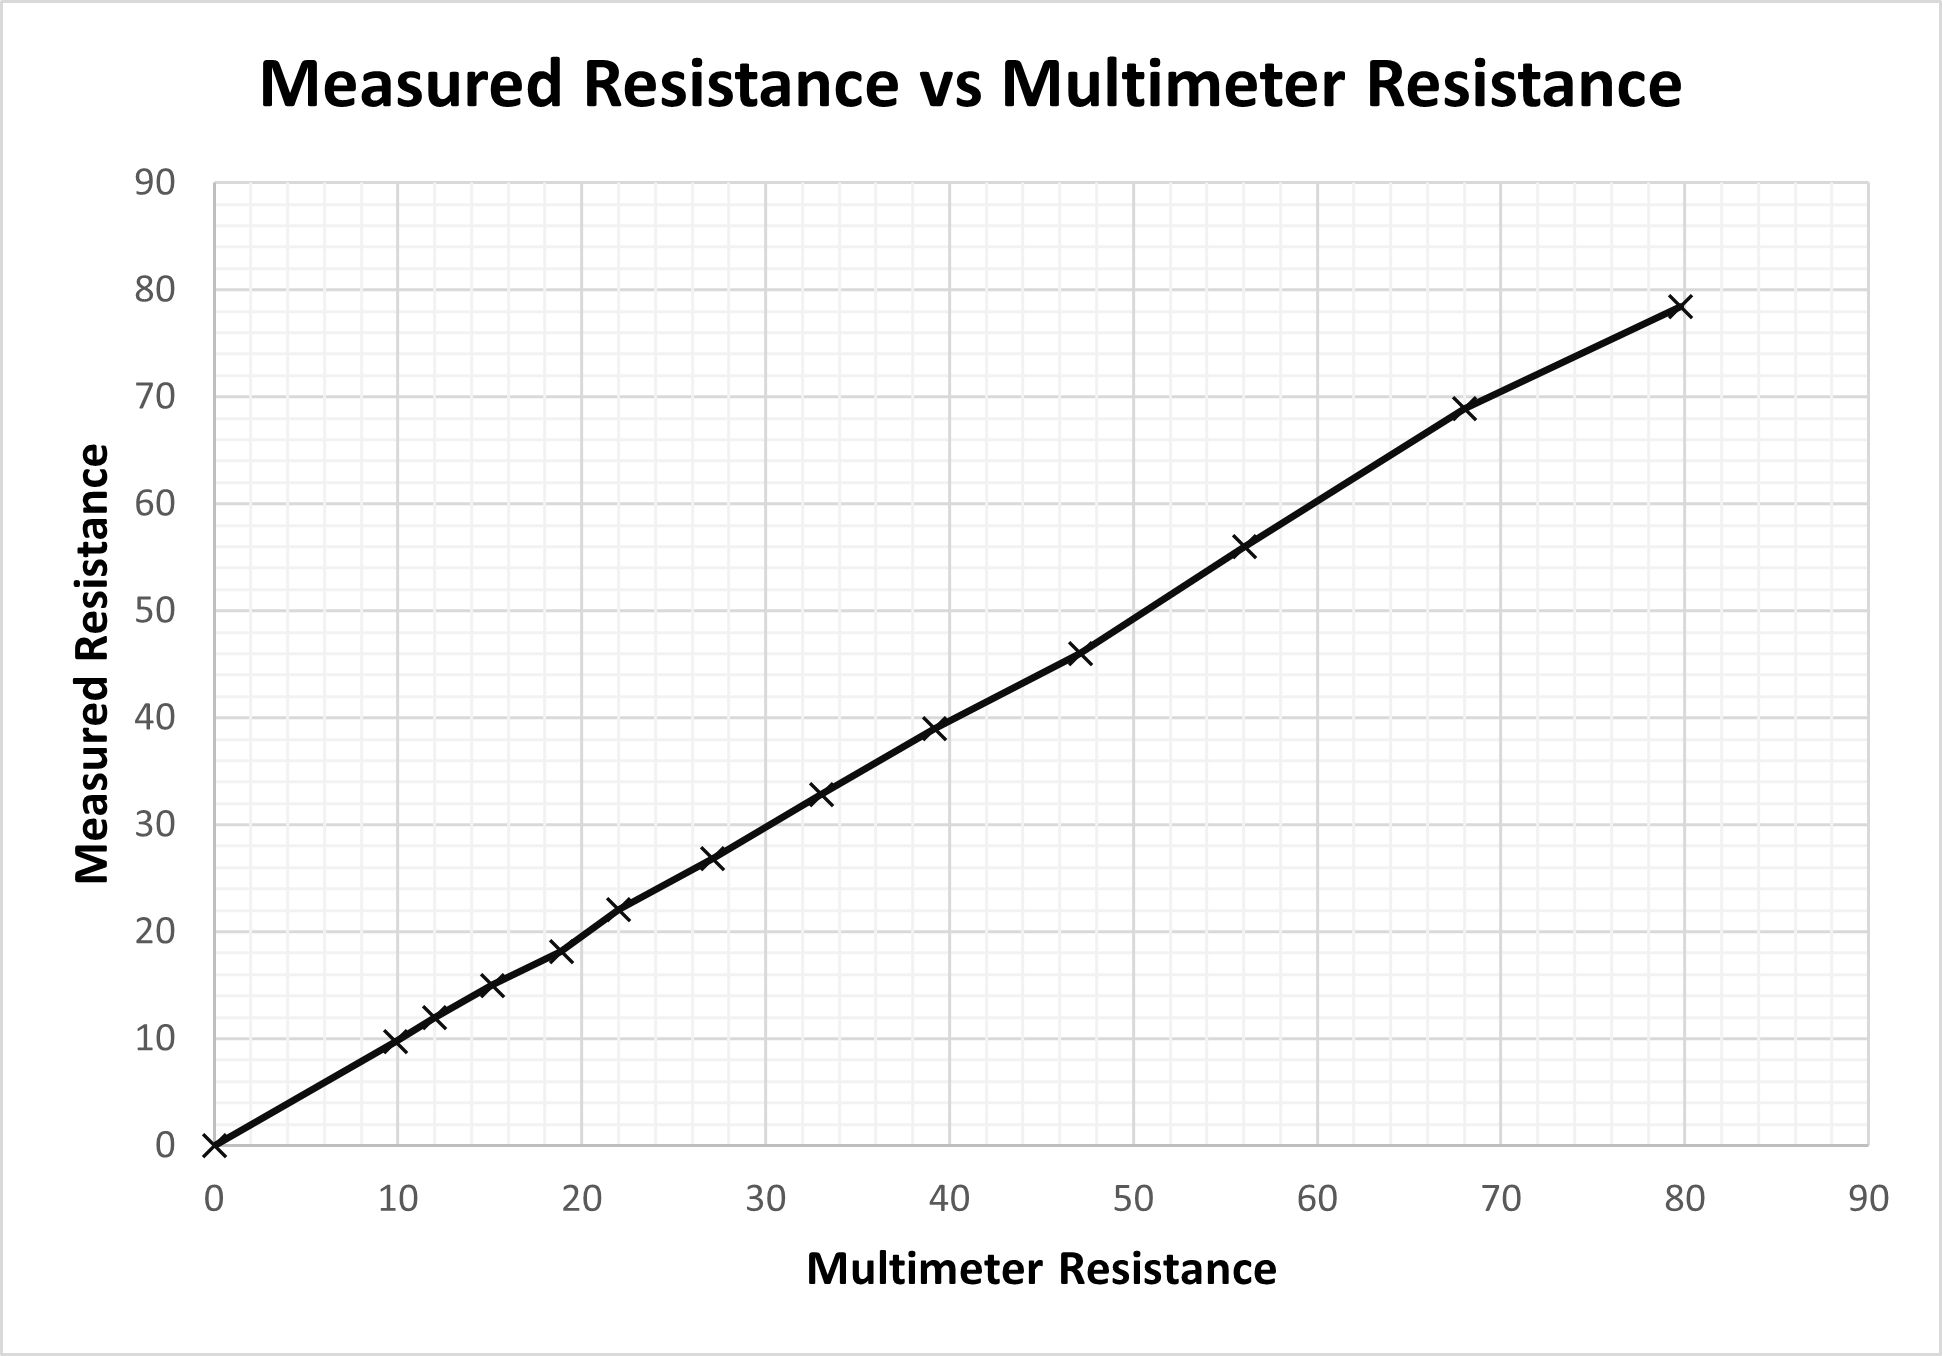
\includegraphics[width=0.7\textwidth]{figures/resistance_measurement_test.png}
    \caption{Resistance Measurement Test via Voltage Sweep}
    \label{fig:resistance_measurement_test}
\end{figure}

For both these tests, voltage calibration via the calibration resistor was done to ensure accurate voltage measurements.

\section{Salinity Testing}
In order for the probe to conduct salinity based tests, it was cast in epoxy as described in Section~\ref{sec:waterproofing}.
Following this a range of tests were conducted, ranging from testing voltage measurements on saline solutions, to measuring salinity via conductivity.

\subsection{Voltage Measurement Accuracy and Repeatability}
In order to get an understanding of how the electrodes interact with saline solutions, a voltage sweep test was conducted multiple times with the same solution.
This was done using the voltage sweep function, mentioned in Section~\ref{sec:uc_program}, with some alterations, allowing for the function to return the raw voltage instead of the conductivity.
The results showed that on the same solution, the the voltage sweep had the same effects.
However, it was noticed that when a volatge reading was taken in quick succession to another there was a slight interference was caused by the water, to counteract this a 1 second delay was introduced between each measurement.
After this delay was added, the interference was no longer observed.

Figure~\ref{fig:repeatability_test} shows voltage sweeps across the same solution on three seperate occasions.
\begin{figure}[H]\label{fig:repeatability_test}
    \centering
    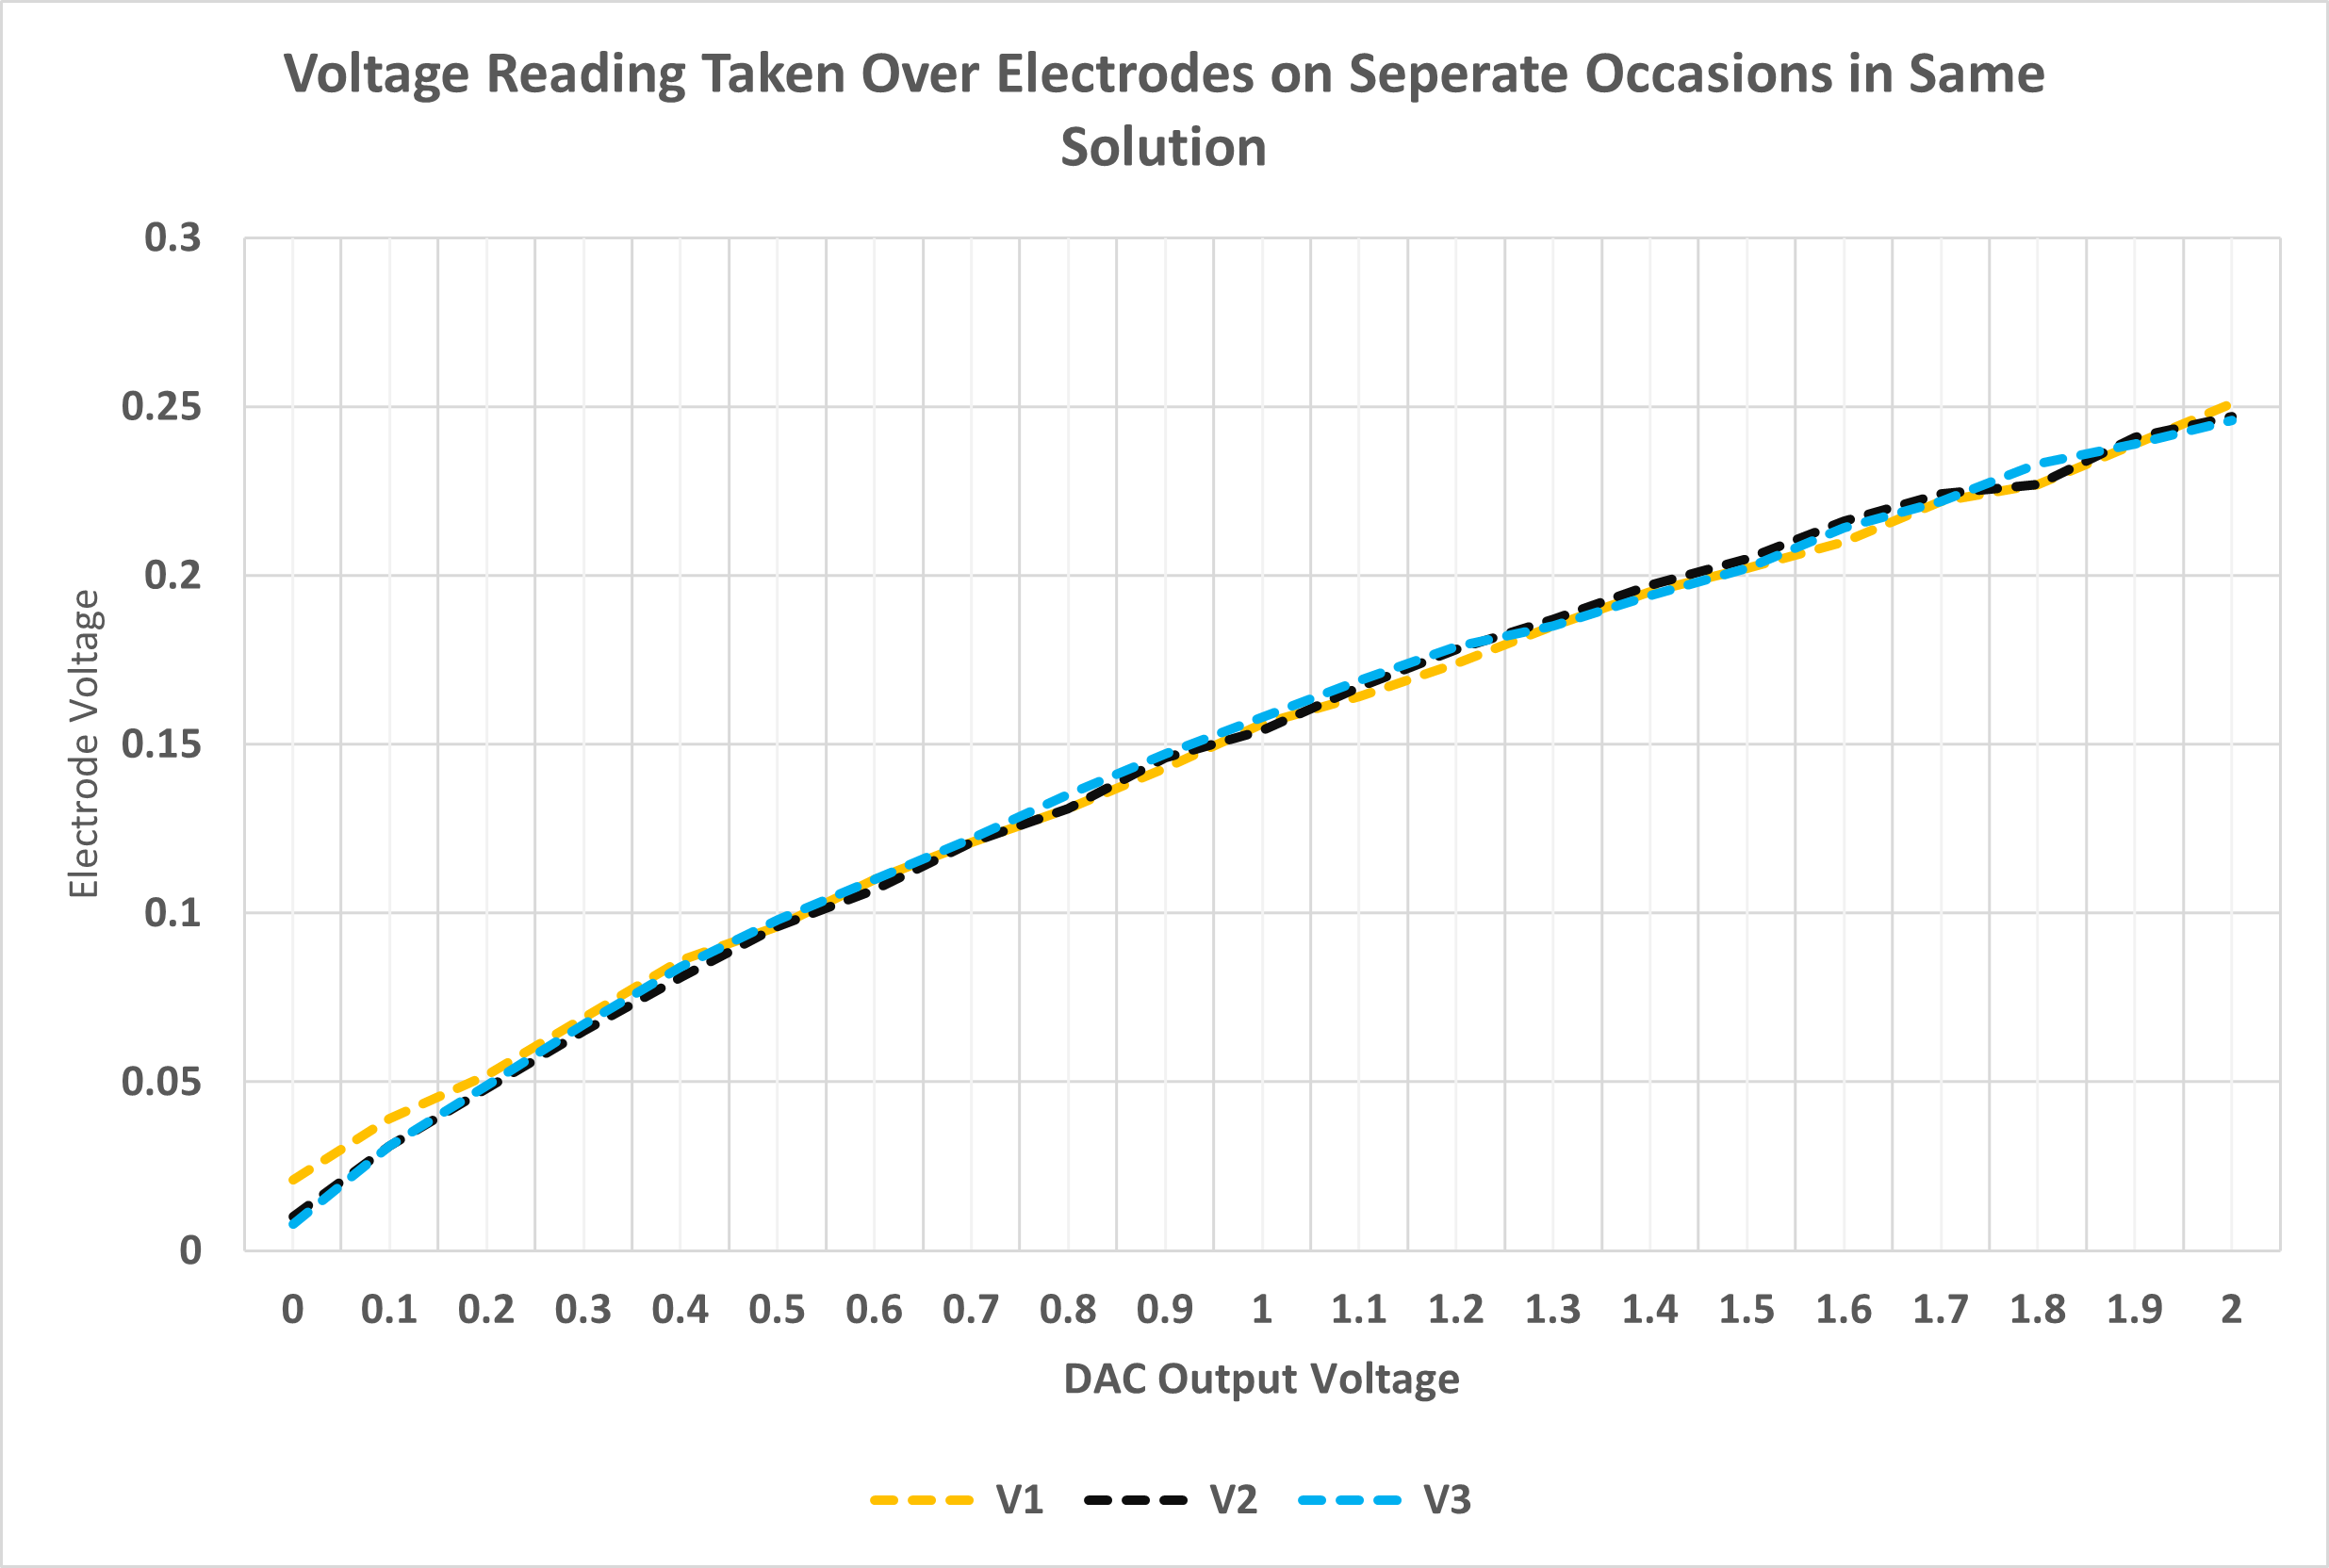
\includegraphics[width=0.7\textwidth]{figures/repeatability_test.png}
    \caption{Repeatability Test Results}
    \label{fig:repeatability_test}
\end{figure}

\subsection{Conductivity and Salinity Measurement}

\subsubsection{Obtaining Conductivity of the Standard Solution}
For the measurement of salinity from conductivity, the conductivity of the standard solution of $35$ \gls{psu} at $15^{\circ}C$ and $0dbar$ must first be obtained.
To evaluate this, both the voltage sweep and single voltage measurements wer taken in a solution at standard conditions.
To achieve these conditions salt was mied into water until the salinity was 34.8 \gls{psu}.
This value was used, as creating a solution of a specific salinity is a time-consuming process, and it was considered close enough for this experiment.
To achieve a temperature of $15^\circ$C the water was cooled in a fridge to $4^\circ$C and then left out until it reached $15^\circ$C.
The salinity was measured using a salinometer.
Once the required conditions were achieved, a voltage sweep from $0-2V$ was done using the previously mentioned voltage sweep function.
As mentioned in Section~\ref{sec:uc_program}, in the voltage sweep description, this returns the conductivity and resistance for each step.
All measurements for this and subsequent tests were conducted at $0dbar$, while using the $100\Omega$ $R_1$ resistor as the measured resistances were between $1-15\Omega$.
The sweep was conducted twice to ensure repeatability.
From this test the average conductivity of the standard solution was found to be $3.53 S/m$, with an average electrode/water resistance of $6.81\Omega$.

Similar results were obtained using single voltage measurements, where multiple readings were taken at one voltage using the DC Single Voltage function, and this was done for voltages of $1-1.5V$.
Here the average resistance was calculated to be $7.39\Omega$ and average conductivity of $3.53 S/m$.
These values correlate well with the expected resistance of $7.55\Omega$.

The Single Voltage Test can be seen in Table~\ref{table:sal_vsingledc}, with a graph illustrating the Voltage vs Resistance, taken from the Voltage Sweep Test, shown in Figure~\ref{fig:sal_vsweepdc}.

\begingroup
    \renewcommand{\arraystretch}{1.8} % increase row height (adjust factor as needed)
    \begin{table}[h!]
        \centering
            \begin{tabular}{|>{\centering\arraybackslash}p{1cm}|
                >{\centering\arraybackslash}m{1cm}|
                >{\centering\arraybackslash}m{1.8cm}|
                >{\centering\arraybackslash}m{2.2cm}|
                >{\centering\arraybackslash}m{3cm}|
                >{\centering\arraybackslash}m{3cm}|
                >{\centering\arraybackslash}m{2cm}|}
            \hline
                \textbf{V IN (V)} & \textbf{Vp AMP (V)} & \textbf{Calib F} & \textbf{Probe V (V)} & \textbf{Resistance ($\Omega$)} & \textbf{Conductivity (mS/cm)} \\ \hline
                1.2 & 1.112 & 0.7786 & 0.078709382 & 7.0195345 & 3.561489724 \\ \hline
                1.2 & 0.721 & 0.7786 & 0.051033691 & 4.4417047 & 3.628469589 \\ \hline
                1.3 & 1.355 & 0.7739 & 0.095330409 & 7.9130471 & 3.159195482 \\ \hline
                1.3 & 1.251 & 0.7739 & 0.088013536 & 7.2619240 & 3.442613812 \\ \hline
                1.4 & 1.312 & 0.7739 & 0.092305164 & 7.0586150 & 3.541770538 \\ \hline
                1.4 & 1.452 & 0.7739 & 0.102154800 & 7.8711082 & 3.176172238 \\ \hline
                1.5 & 1.573 & 0.7745 & 0.110753500 & 7.9721993 & 3.135897151 \\ \hline
                1.5 & 1.359 & 0.7745 & 0.095685955 & 6.8137148 & 3.669007482 \\ \hline
                1.6 & 2.211 & 0.7724 & 0.155525240 & 10.745988 & 3.226447904 \\ \hline 
                1.6 & 1.451 & 0.7724 & 0.101886582 & 6.8009925 & 3.675934042 \\ \hline
                \textbf{Mean} &  &  &  & \textbf{7.38991} & \textbf{3.531706371} \\ \hline
            \end{tabular}
        \caption{Table for Standard Salinity Solution Test}
        \textit{Note: For this test an R1 resistance of 100$\Omega$ was used.}
        \label{table:sal_vsingledc}
    \end{table}
\endgroup

%TODO table sweep or smth
\begin{figure}[H]\label{fig:sal_vsweepdc}
    \centering
    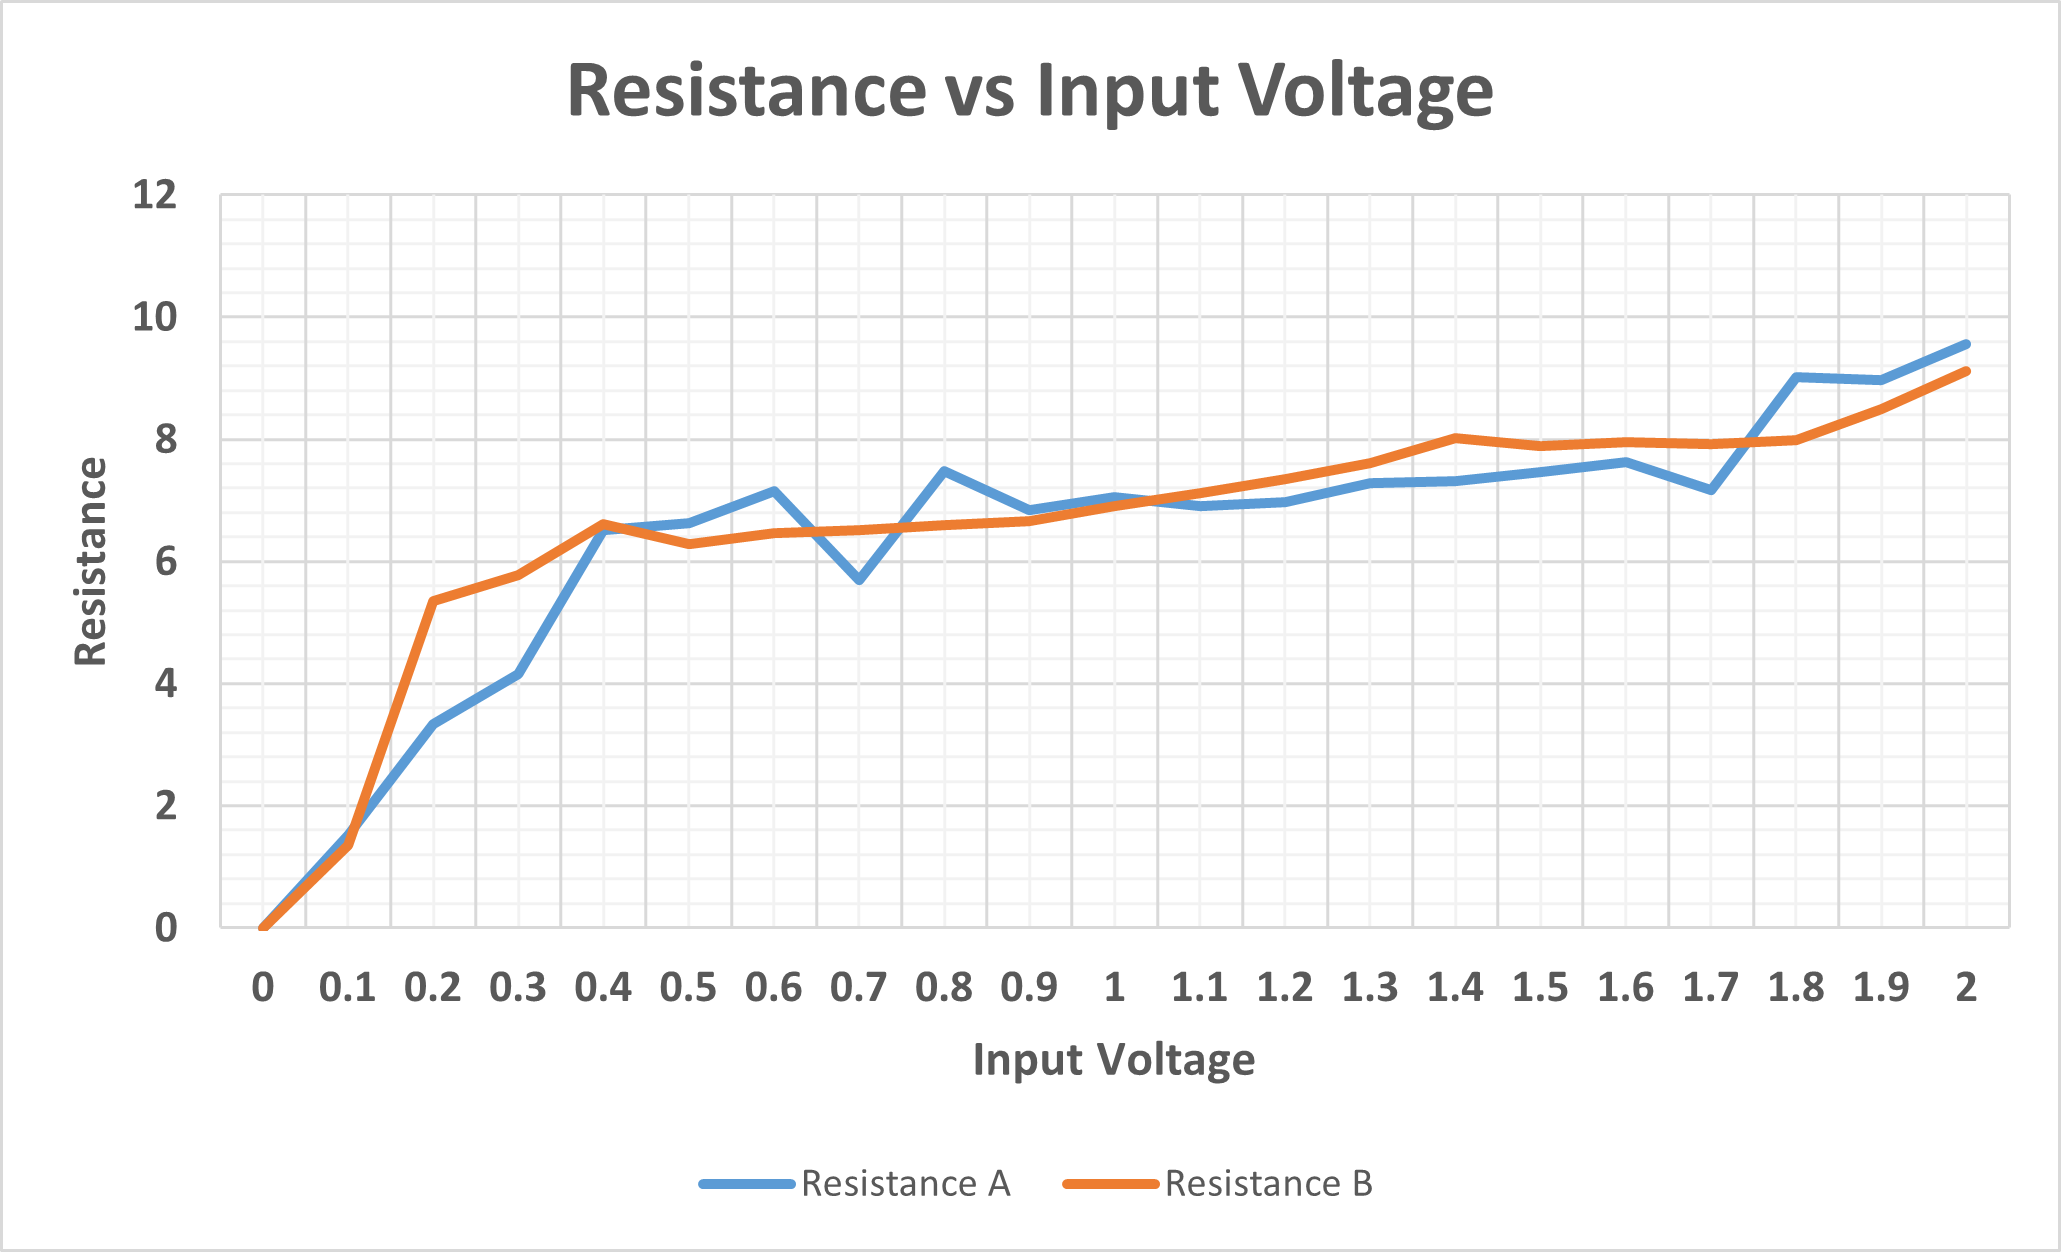
\includegraphics[width=0.7\textwidth]{figures/sal_vsweep.png}
    \caption{Volatge Sweep Test Showing Resistance vs Input Voltage}
    \label{fig:sal_vsweepdc}
\end{figure}

\subsubsection{Measuring Salinity of Sample Solutions}
Once the conductivity of the standard solution was found, the PSS-78 salinity equations could be used to find the salinity of sample solutions.
The both the DC Single Voltage and DC Sweep Voltage functions were updated to return the salinity of a measured solution.
For the DC Single Voltage Test, a voltage of $1.4V$ was found to return the most accurate value.
Using these methods salinity of solutions were tested against a salinometer and compared.
The comparisons for the Single Voltage test can be seen in Table~\ref{table:salinity_measurements}.

\begingroup
    \renewcommand{\arraystretch}{1.8} % increase row height (adjust factor as needed)
    \begin{table}[H]
        \centering
            \begin{tabular}{|>{\centering\arraybackslash}p{1.5cm}|
                >{\centering\arraybackslash}m{1cm}|
                >{\centering\arraybackslash}m{1.5cm}|
                >{\centering\arraybackslash}m{2cm}|
                >{\centering\arraybackslash}m{2.5cm}|
                >{\centering\arraybackslash}m{3cm}|
                >{\centering\arraybackslash}m{2cm}|}
            \hline
                \textbf{Salinity (PSU)} & \textbf{T (°C)} & \textbf{Probe Voltage} & \textbf{Calib Factor} & \textbf{Corrected Voltage} & \textbf{Resistance ($\Omega)$} & \textbf{Calculated Salinity} \\ \hline
                34.8  & 15    & 0.119 & 0.7739 & 0.0920941 & 7.041339901  & 35    \\ \hline
                30.1  & 15    & 0.145 & 0.7745 & 0.1123025 & 8.721186459  & 28.02 \\ \hline
                23.74 & 15    & 0.188 & 0.7601 & 0.1428988 & 11.36732667  & 20.71 \\ \hline
                23.72 & 24.31 & 0.108 & 0.7687 & 0.0830196 & 6.30378402   & 25.82 \\ \hline
                32.65 & 24.27 & 0.084 & 0.7693 & 0.0646212 & 4.839166235  & 35.15 \\ \hline
                15.8  & 20    & 0.197 & 0.7772 & 0.1531084 & 12.27920695  & 14.95 \\ \hline
                20.4  & 20    & 0.163 & 0.7779 & 0.1267977 & 9.958959389  & 18.75 \\ \hline
                17.26 & 20    & 0.197 & 0.7799 & 0.1536403 & 12.32712354  & 14.83 \\ \hline
            \end{tabular}
        \caption{Table for Sample Salinity Test}
        \textit{Note: T denotes temperature, Calib Factor denotes Calibration Factor.}
        \label{table:salinity_measurements}
    \end{table}
\endgroup

From these measured values it can be seen that the probe has a measuring accuracy of approximately $\pm3.5$ \gls{psu}.


\section{EIS and Machine Learning}
As mentioned 



